\section{Problem}
\markright{Problem}

This program demonstrates the four properties of a class through a sensor example.

\textbf{Abstraction:} The abstract base class \texttt{Sensor} defines a common interface for all sensors. It declares the pure virtual method \texttt{display()} and hides common details such as the sensor name. Concrete sensor classes must implement \texttt{display()}, which makes the design easier to extend and maintain.

\textbf{Encapsulation:} The derived classes \texttt{TemperatureSensor} and \texttt{DistanceSensor} store their values in private members (\texttt{temperature} and \texttt{distance}). These values cannot be changed directly from outside the class. Instead, public \texttt{setValue()} and \texttt{getValue()} methods provide controlled access.

\textbf{Inheritance:} \texttt{TemperatureSensor} and \texttt{DistanceSensor} inherit from \texttt{Sensor}. This relationship allows them to reuse the common sensor interface and share the \texttt{name} field from the base class.

\textbf{Polymorphism:} In \texttt{main()}, an array of \texttt{Sensor*} pointers stores addresses of the derived objects. The loop calls \texttt{sensors[i]->display()} on each pointer. Because \texttt{display()} is virtual, the correct derived implementation runs at runtime, showing polymorphic behavior.

Both derived classes also use overloaded \texttt{setValue()} methods to accept either integer or double input. While this is compile-time polymorphism, the main runtime polymorphism in the program comes from the virtual \texttt{display()} function.

\subsubsection{Code}
\begin{lstlisting}[language=C++, numbers=left]
#include <iostream>
#include <string>

using namespace std;

// Abstract class (Abstraction)
class Sensor {
protected:
    string name;

public:
    Sensor(string n) {
        name = n;
    }

    // Pure virtual function
    virtual void display() = 0;

    virtual ~Sensor() {}
};

// Inheritance + Encapsulation
class TemperatureSensor : public Sensor {
private:
    double temperature;

public:
    TemperatureSensor(string n) : Sensor(n) {
        temperature = 0;
    }

    // Function overloading
    void setValue(int t) {
        temperature = t;
    }

    void setValue(double t) {
        temperature = t;
    }

    double getValue() {
        return temperature;
    }

    // Polymorphism
    void display() override {
        cout << name << " Temperature: "
             << temperature << " degree C" << endl;
    }
};

class DistanceSensor : public Sensor {
private:
    double distance;

public:
    DistanceSensor(string n) : Sensor(n) {
        distance = 0;
    }

    // Function overloading
    void setValue(int d) {
        distance = d;
    }

    void setValue(double d) {
        distance = d;
    }

    double getValue() {
        return distance;
    }

    void display() override {
        cout << name << " Distance: "
             << distance << " cm" << endl;
    }
};

int main() {

    TemperatureSensor temp("LM35");
    DistanceSensor dist("Ultrasonic");

    temp.setValue(36.5);   // double version
    dist.setValue(125);    // int version

    // Array of pointers (Pointer + Array)
    Sensor* sensors[2];

    sensors[0] = &temp;
    sensors[1] = &dist;

    cout << "=== Sensor Readings ===\n\n";

    // Polymorphism in action
    for (int i = 0; i < 2; i++) {
        sensors[i]->display();
    }

    return 0;
}
\end{lstlisting}

\subsubsection{Output}
\begin{figure}[H]
  \centering
  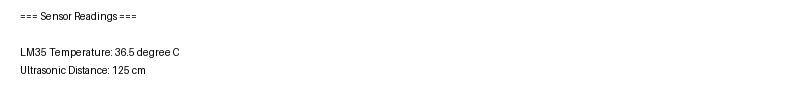
\includegraphics[width=0.8\textwidth]{lab-04/assets/output.png}
  \caption{Program output showing temperature and distance sensor readings via polymorphic base-class pointers.}
\end{figure}
